% SETUP
\documentclass{article}
\usepackage{amsmath}
\usepackage{amsthm}
\usepackage{amssymb}
\usepackage{hyperref}
\usepackage{graphicx}
\graphicspath{{Images/}}
\usepackage[
    left=2.15cm,
    right=2.15cm,
    top=1.90cm,
    bottom=1.90cm
]{geometry}

\title{3,220: Data Analytics I: Statistik (VWL)}
\author{Leroy Zahno}
\date{Autumn Semester 2026}

\makeatletter
\renewcommand{\maketitle}{%
  \begin{center}
    {\LARGE \@title \par}
    \vspace{1em}
    {\large \@author \par}
    \vspace{1em}
    {\large \@date \par}
  \end{center}
}
\makeatother

% CUSTOM STYLES
\newtheorem{theorem}{Theorem}

\theoremstyle{definition}
\newtheorem{definition}{Definition}

\theoremstyle{exercise}
\newtheorem{exercise}{Exercise}

\theoremstyle{solution}
\newtheorem{solution}{Solution}

\theoremstyle{lemma}
\newtheorem{lemma}{Lemma}

\begin{document}

\maketitle
\tableofcontents

% NEW SECTION
\section{Daten und deskriptive Statistik}
\subsection{Lernziele}
Nach dieser Vorlesung hat man gelernt, wie die verschiedenen Datentypen unterschieden werden; die Konzepte der beschreibenden Statistik in praxisorientierten Datenbeispielen angewandt werden; Daten übersichtlich aufbereitet und grafisch zur Interpretation darstellbar gemacht werden. 

\subsection{Skalenniveau von Merkmalen}
Eine statistische Grundgesamtheit besteht aus Einheiten mit denselben Ausprägungen sachlicher, zeitlicher und räumlicher Identifikationsmerkmale. Das Skalenniveau hat Einfluss sowohl auf die Erhebbarkeit als auch auf die Wahl der Auswertungsmethode und damit auf den Informationsgehalt des Messergebnisses. Wir unterscheiden zwischen den nachfolgenden Skalenarten: Qualitativ an der Nominalskala, komparativ an der ordinalskala und quantitativ an den Intervall- und Verhältnisskalen.

\subsection{Verteilungen und Lage- und Streuungsparameter}
\begin{theorem}[Symmetrische Verteilung]
Im Falle einer \textit{symmetrischen Verteilung} nehmen Mittelwert, Median und Modus den gleichen Wert an. Eine symmetrische Verteilung besitzt eine Schiefe von $0$ (siehe Figure 1). 
\end{theorem}

\begin{definition}[Sehne]
In einem Zufallsexperiment ist eine Sehne eine gerade Verbindungslinie zwischen zwei Punkten auf dem Rand eines geometrischen Objekts (meistens eines Kreises), wobei diese beiden Punkte durch Zufall ausgewählt werden (Gemini, 2026).
\end{definition}

\begin{definition}[Ergebnismenge]
Eine Ergebnismenge ist eine Menge von Mengen. Für endliche Ergebnismengen \(S\) wählt man meist

\[ E(S)=\mathcal{P}(S)=\{A|A\subseteq S\},\]
also die Potenzmenge von \(S\).
\end{definition}

\begin{definition}[Laplace-Experiment]
Ein Zufallsexperiment mit endlich vielen gleichwahrscheinlichen Elementarereignissen heisst Laplace-Experiment. Eine Anwendung dessen nennt man einen \textit{L-Versuch}.

\end{definition}

\begin{definition}[Schiefe]
Die Schiefe einer Verteilungsfunktion beschreibt die Tendenz der Verteilung, extreme Werte links und rechts am Ende der Verteilungsfunktion mit überdurchschnittlicher Wahrscheinlichkeit anzunehmen.
\end{definition}

\begin{figure}[ht]
\centering

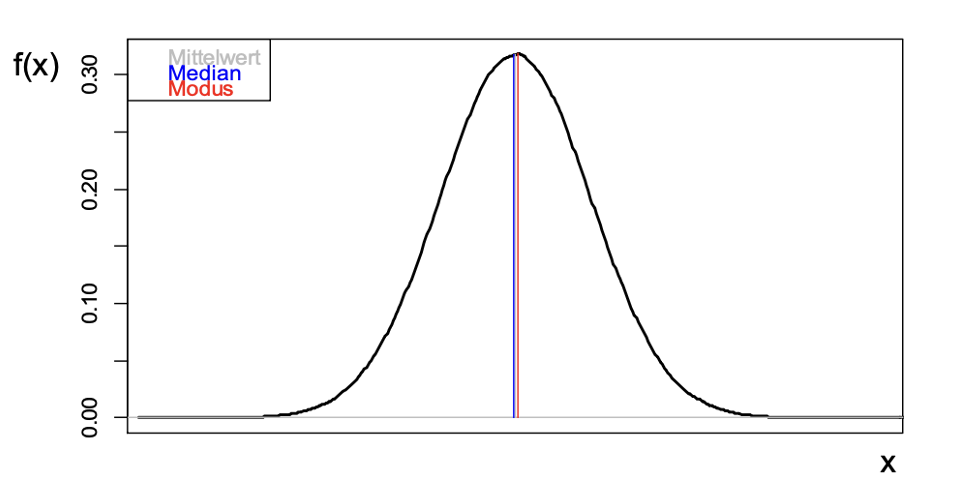
\includegraphics[width=\textwidth]{schiefe.png}

\caption{Lageparameter bei symmetrischer Verteilungsfunktion}
\end{figure}

\begin{theorem}[Charakterisierung der Schiefe einer Verteilungsfunktion]
Eine Verteilung mit positiver Schiefe heisst \textit{linkssteil bzw. rechtsschief} und bedeutet, dass der Mittelwert grösser als der Median grösser als der Modus ist. Eine Verteilung mit negativer Schiefe heisst \textit{rechtssteil bzw. linksschief} und bedeutet, dass der Mittelwert kleiner als der Median kleiner als der Modus ist.
\end{theorem}

\begin{definition}[Kurtosis]
Die Kurtosis drückt aus, ob die Verteilung im Vergleich zur Normalverteilung, bzw. zur mesokurtischen Verteilung, eher schmalgipflig, bzw. leptokurtisch (für $\textgreater 0$) oder breitgipflig, bzw. platykurtisch (für $\textless 0$) ist (Siehe Figure 2).
\end{definition}

\begin{figure}[ht]
\centering

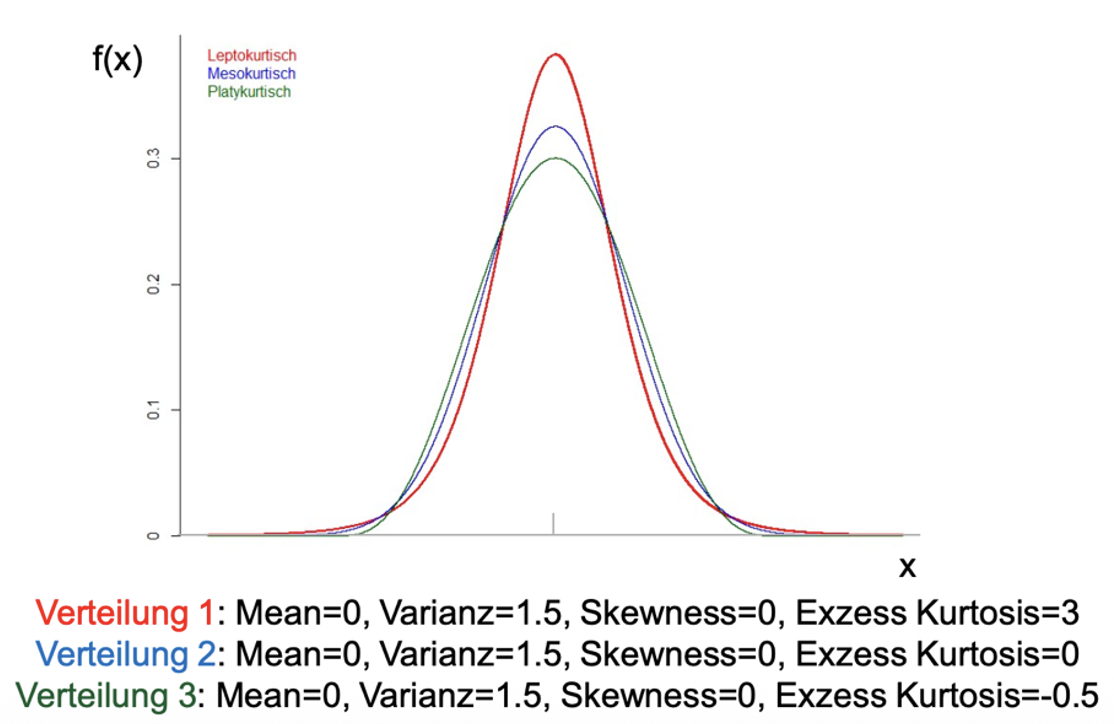
\includegraphics[width=\textwidth]{kurtosis.png}

\caption{Gleiche Verteilungsfunktion mit divergierender Kurtosis.}
\end{figure}

\begin{definition}[Mittlere Absolute Abweichung]
Die Mittlere absolute Abweichung (MAD) kann anhand einer Grundgesamtheit (Population) oder Stichprobe (Subset der Grundgesamtheit) errechnet werden:

\[ \text{Grundgesamtheit:} \quad MAD=\frac{\sum_{i=1}^{N}|X_i-\mu|}{N} \]
\[ \text{Stichprobe:} \quad MAD_s=\frac{\sum_{i=1}^{n}|x_i-\overline{x}|}{n-1} \]

\end{definition}

% NEW SECTION

\section{Korrelation vs. Kausalität}
\subsection{Lernziele}
Nach dieser Vorlesung hat man gelernt, wie man den Zusammenhang zwischen Daten mit Hilfe von Korrelation misst und interpretiert; man zwischen den Konzepten der Korrelation und Kausalität unterscheidet und diese anhand konkreter, praxisorientierter Beispiele anwendet.

\subsection{Korrelation vs. Kausalität}
Werden Paare von Beobachtungsdaten erhoben, kann das Datenmaterial so beschaffen sein, dass zwischen den Paaren ein statistischen Zusammenhang, also eine Korrelation, errechnet werden kann. Ob Dabei ein kausaler Zusammenhang besteht, ist damit noch nicht sichergestellt.

\begin{definition}[Korrelation]
Korrelation bedeutet, dass ein Zusammenhang zwischen Variablen, jedoch nicht zwangsläufig ein Ursache-Wirkungs-Zusammenhang, existiert.
\end{definition}

\begin{definition}[Kausalität]
Kausalität bedeutet, dass zwei Variablen in einem Ursachen-Wirkungs-Zusammenhang zueinander stehen.
\end{definition}

\subsection{Korrelationskoeffizient}
\begin{definition}[Korrelationskoeffizient]
Der Korrelationskoeffizient \(\rho\) liefert ein Mass für die Stärke der Richtung des Zusammenhangs zwischen zwei metrisch messbaren Variablen wie etwa zwischen Körpergrösse und Einkommen oder zwischen Öl-Preis und der Entwicklung eines Aktienindexes. Wir machen folgende Feststellungen:

\[ \rho = -1 \quad\ \text{Perfekte negative Korrelation,}\]
\[ \rho = 0 \quad \text{Unkorreliertheit,}\]
\[ \rho = 1 \quad \text{Perfekte positive Korrelation,}\]
\[ -1 < \rho < 1 \quad \text{Korrelation.}\]
\end{definition}

\subsection{Kovarianz}
Der Korrelationskoeffizient wird über die Kovarianz bestimmt. Das nicht-standardisierte Mass der Kovarianz errechnet sich aus der Summe aller Produkte der Mittelwertabweichungen beider Datenpunkte.
\[ \rho=\frac{Kovarianz(X,Y)}{\sigma_x\sigma_y} \qquad Kovarianz_{x,y}=\frac{\sum_{i=1}^N(X_i-\mu_x)(Y_i-\mu_y)}{N} \]

Für Beobachtungen in Stichproben werden Mittelwert und Standardabweichung durch die entsprechenden Stichprobenvarianzen bei der Berechnung ersetzt. Aus \(\rho\) wird entsprechend \(r\) und aus \((X_i,\mu_x)\) werden \((x_i,\overline{x})\).

\subsection{Portfolio-Optimierung}

\[ Sharpe Ratio = \frac{risk premium}{standard deviation}=\frac{r-r_f}{\sigma} \]

% NEW SECTION

\section{Wahrscheinlichkeitstheorie}
\subsection{Lernziele}
Nach dieser Vorlesung hat man gelernt, wie die Grundkonzepte der Wahrscheinlichkeitstheorie in Beispielen angewendet werden; die Grundkonzepte der Wahrscheinlichkeitstheorie anhand von Venn-Diagrammen dargestellt werden; das Konzept der bedingten Wahrscheinlichkeit mit Hilfe von Baudiagrammen visualisiert werden kann.

\subsection{Grundbegriffe}

\begin{definition}[Ereignis, Ereignismenge, Ergebnisraum]
Alle Ereignisse eines Zufallsexperimentes mit dem Ergebnisraum \(S\) bilden die dazugehörige Ereignismenge \(E(S)\). Die Ereignismenge ist die Menge von Teilmengen im Ergebnisraum. Ein Ereignis ist eine Teilmenge eines Ergebnisraums. Ein Elementarereignis ist ein Element eines Ereignisses.
\end{definition}

\begin{definition}[Bedingte Wahrscheinlichkeit]
Seien \(A\) und \(B\) zwei Ereignisse eines gegebenen Wahrscheinlichkeitsraums. Die bedingte Wahrscheinlichkeit \(A\) unter der Bedingung \(B\) ist definiert als
\[
P(A|B)=\frac{(A\cap B)}{P(B)}, \text{ für } P(B)>0
\]
und undefiniert für \(P(B)=0\).
\end{definition}

\begin{theorem}[Multiplikationssatz]
Die Wahrscheinlichkeit, dass zwei Ereignisse \(A\) und \(B\) gleichzeitig eintreten, beträgt
\[
(A\cap B)=P(A)\cdot P(B|A)
\]
oder
\[
(B\cap A)=P(B) \cdot P(A|B).
\]
\end{theorem}

\begin{definition}[Stochastisch unabhängig, unabhängig]
Zwei Ereignisse \(A\) und \(B\) heissen (stochastisch) unabhängig, wenn
\[
P(A|B)=P(A), P(B|A)=P(B).
\]
\end{definition}

\begin{theorem}[Multiplikationssatz für unabhängige Ereignisse]
Sind zwei Elementarereignisse \(A\) und \(B\) unabhängig, dann ist
\[
P(A\cap B)=P(A)\cdot P(B).
\]
\end{theorem}


\begin{definition}[Ereignis und Komplementärereignis]
Ein Ereignis ist jede beliebige Teilmenge \(A\) des Ereignisraumes $\Omega$. Ein Ereignis tritt dann ein, oder wird realisiert, wenn ein in ihm enthaltenes Elementarereignis $\omega$ eintritt. Für ein Ereignis $A$ ist das Komplementär-Ereignis "nicht A" $\overline{A}$ definiert als die Menge aller Elementarereignisse des Zustandsraums $\Omega$, die nicht in $A$ enthalten sind. Wir schreiben $\overline{A}=\Omega \backslash A$.
\end{definition}

\begin{definition}[Wahrscheinlichkeitsbegriffe]
Der \textit{klassische Wahrscheinlichkeitsbegriff} definiert die Wahrscheinlichkeit als das Verhältnis der Anzahl günstiger Fälle zur Anzahl aller gleichmöglichen Fälle bei einem Zufallsexperiment.  Der \textit{statistische Wahrscheinlichkeitsbegriff} orientiert sich am Gesetz der Grossen Zahlen und entspricht der Häufigkeit mit der ein Ergebnis bei einer entsprechend grossen Anzahl von Versuchen auftritt. Der \textit{subjektive Wahrscheinlichkeitsbegriff} ist das Mass für den Grad der Überzeugtheit der Richtigkeit einer Aussage.
\end{definition}

\begin{theorem}[Die kolmogorovschen Axiome]
Die Wahrscheinlichkeit $\mathbb{P}(A)$ ist eine eindeutig bestimmte, nichtnegative, reelle Zahl, die höchstens gleich eins sein kann. $0\leq \mathbb{P}(A)\leq 1.$ Das sichere Ereignis besitzt eine Wahrscheinlichkeit eins. $\mathbb{P}(\Omega)=1$ mit $\Omega=\{A_1,A_2,...,A_n\}.$ Für zwei disjunkte Ereignisse $A_1, A_2$ gilt $\mathbb{P}(A_1 \cup A_2)=\mathbb{P}(A_1)+\mathbb{P}(A_2).$ Für jedes Ereignis $A$ gilt $\mathbb{P}(\overline{A})=1-\mathbb{P}(A).$ Die Wahrscheinlichkeit eines unmöglichen Ereignisses $\emptyset$ entspricht $\mathbb{P}(\emptyset)=1-\mathbb{P}(\Omega)=0.$

\end{theorem}

\subsection{Kombinatorik}

\begin{definition}[Fakultät]
Sein $n$ eine positive ganze Zahl. Die Fakultät von $n$, geschrieben als $n!$ (lies "n Fakultät"), ist definiert als
\[ n!=n\cdot (n-1) \cdot (n-2) \cdot ... \cdot 2 \cdot 1 \quad \text{und} \quad 0! = 1.\]
\end{definition}

\begin{theorem}[Anzahl von Permutationen einer endlichen Menge]
Sei $A=\{a_1,...,a_n\}$ eine endliche Menge. Die Anzahl von Permutationen von $A$ ist
\[P(n)=n!.\]
\end{theorem}

\begin{theorem}[Grenzwert einer geometrischen Reihe]
Eine unendliche geometrische Reihe in dieser Form kann wie folgt berechnet werden

\[ \sum_{i=1}^{\infty}\mathbb{P}(P_{3,i})=\mathbb{P}(P_{3,1})+\mathbb{P}(P_{3,2})+\mathbb{P}(P_{3,3})+... \]
\[ =.5^3+.5^6+.5^9 +... \]
\[ =\frac{q}{1-q}=\frac{.5^3}{1-.5^3}=\frac{1}{7}, \]
wobei \(q\) der quotient zweier aufeinander folgenden Glieder der Reihe ist.

\end{theorem}

% NEW SECTION

\section{Zufallsvariablen und Diskrete Verteilungen}
\subsection{Lernziele}
Nach dieser Vorlesung hat man gelernt, wie man mit dem Konzept der Zufallsvariable den Erwartungswert und die Varianz einer diskreten Verteilung berechnen kann; man diskrete Verteilungen durch Verteilungsfunktionen visuell darstellen kann; und wann bestimmte diskrete Verteilungen angewendet werden sollen.

\begin{definition}[Bernoulli-Experiment]
Ein Zufallsexperiment, das lediglich zwei sich gegenseitig ausschliessende Ereignisse $A$ und $\overline{A}$ als mögliche Ergebnisse besitzt, bzw. dessen Ausgang nur in Bezug auf das Eintreten oder Nicht-Eintreten dieser Ergebnisse formuliert wird, nennen wir ein $\textit{Bernoulli-Experiment}$. Eine Folge aus mehreren Bernoulli-Experimenten wird als $\textit{Bernoulli-Kette}$ bezeichnet. 
\end{definition}

\subsection{Binomialverteilung}
\begin{definition}[Binomialverteilung, Stichprobe mit Zurücklegen]
Die Wahrscheinlichkeitsverteilung einer Zufallsvariablen $X$, die beschreibt, wie oft ein bestimmtes Ereignis $\omega$ in einer Bernoulli-Kette auftritt, nennen wir eine $\textit{Binomialverteilung}$. Die Binomialverteilung ist eindeutig durch die Länge der Bernoulli-Kette $n$ und durch die Eintrittswahrscheinlichkeit vom Elementarereignis \(\pi\) bestimmt. Für $n=0,...,n$ ergibt sich die Wahrscheinlichkeitsfunktion wie folgt:

\[f_X(x) =\mathbb{P}[X=x]= \begin{pmatrix} n \\ x \end{pmatrix} \pi^x(1-\pi)^{n-x} \]
\[\Leftrightarrow f_X(x) = \frac{n!}{x!(n-x)!}\pi^x(1-\pi)^{n-x},\]

wobei \(x\) die Anzahl ist, von der wir die Wahrscheinlichkeit suchen, dass \(\omega\) so oft eintrifft. Diese Verteilung wird als Binomialverteilung mit den Parametern $n \geq 1$ und $\pi \in (0,1)$ bezeichnet, und wir schreiben $X \sim$ Bin$(n,\pi)$, um anzugeben, dass $X$ binomialverteilt ist. Es gibt also \(n\) Ereignisse, die je mit einer Wahrscheinlichkeit von \(\pi\) eintreffen können. Die Binomialverteilung hat folgende Eigneschaften: 

\[\mu = \mathbb{E}(x)=n\pi\]
\[\text{Var}[X]=\sigma^2=\mathbb{E}[(x-\mu)^2]=n\pi(1-\pi)\]

\begin{figure}[ht]
\centering

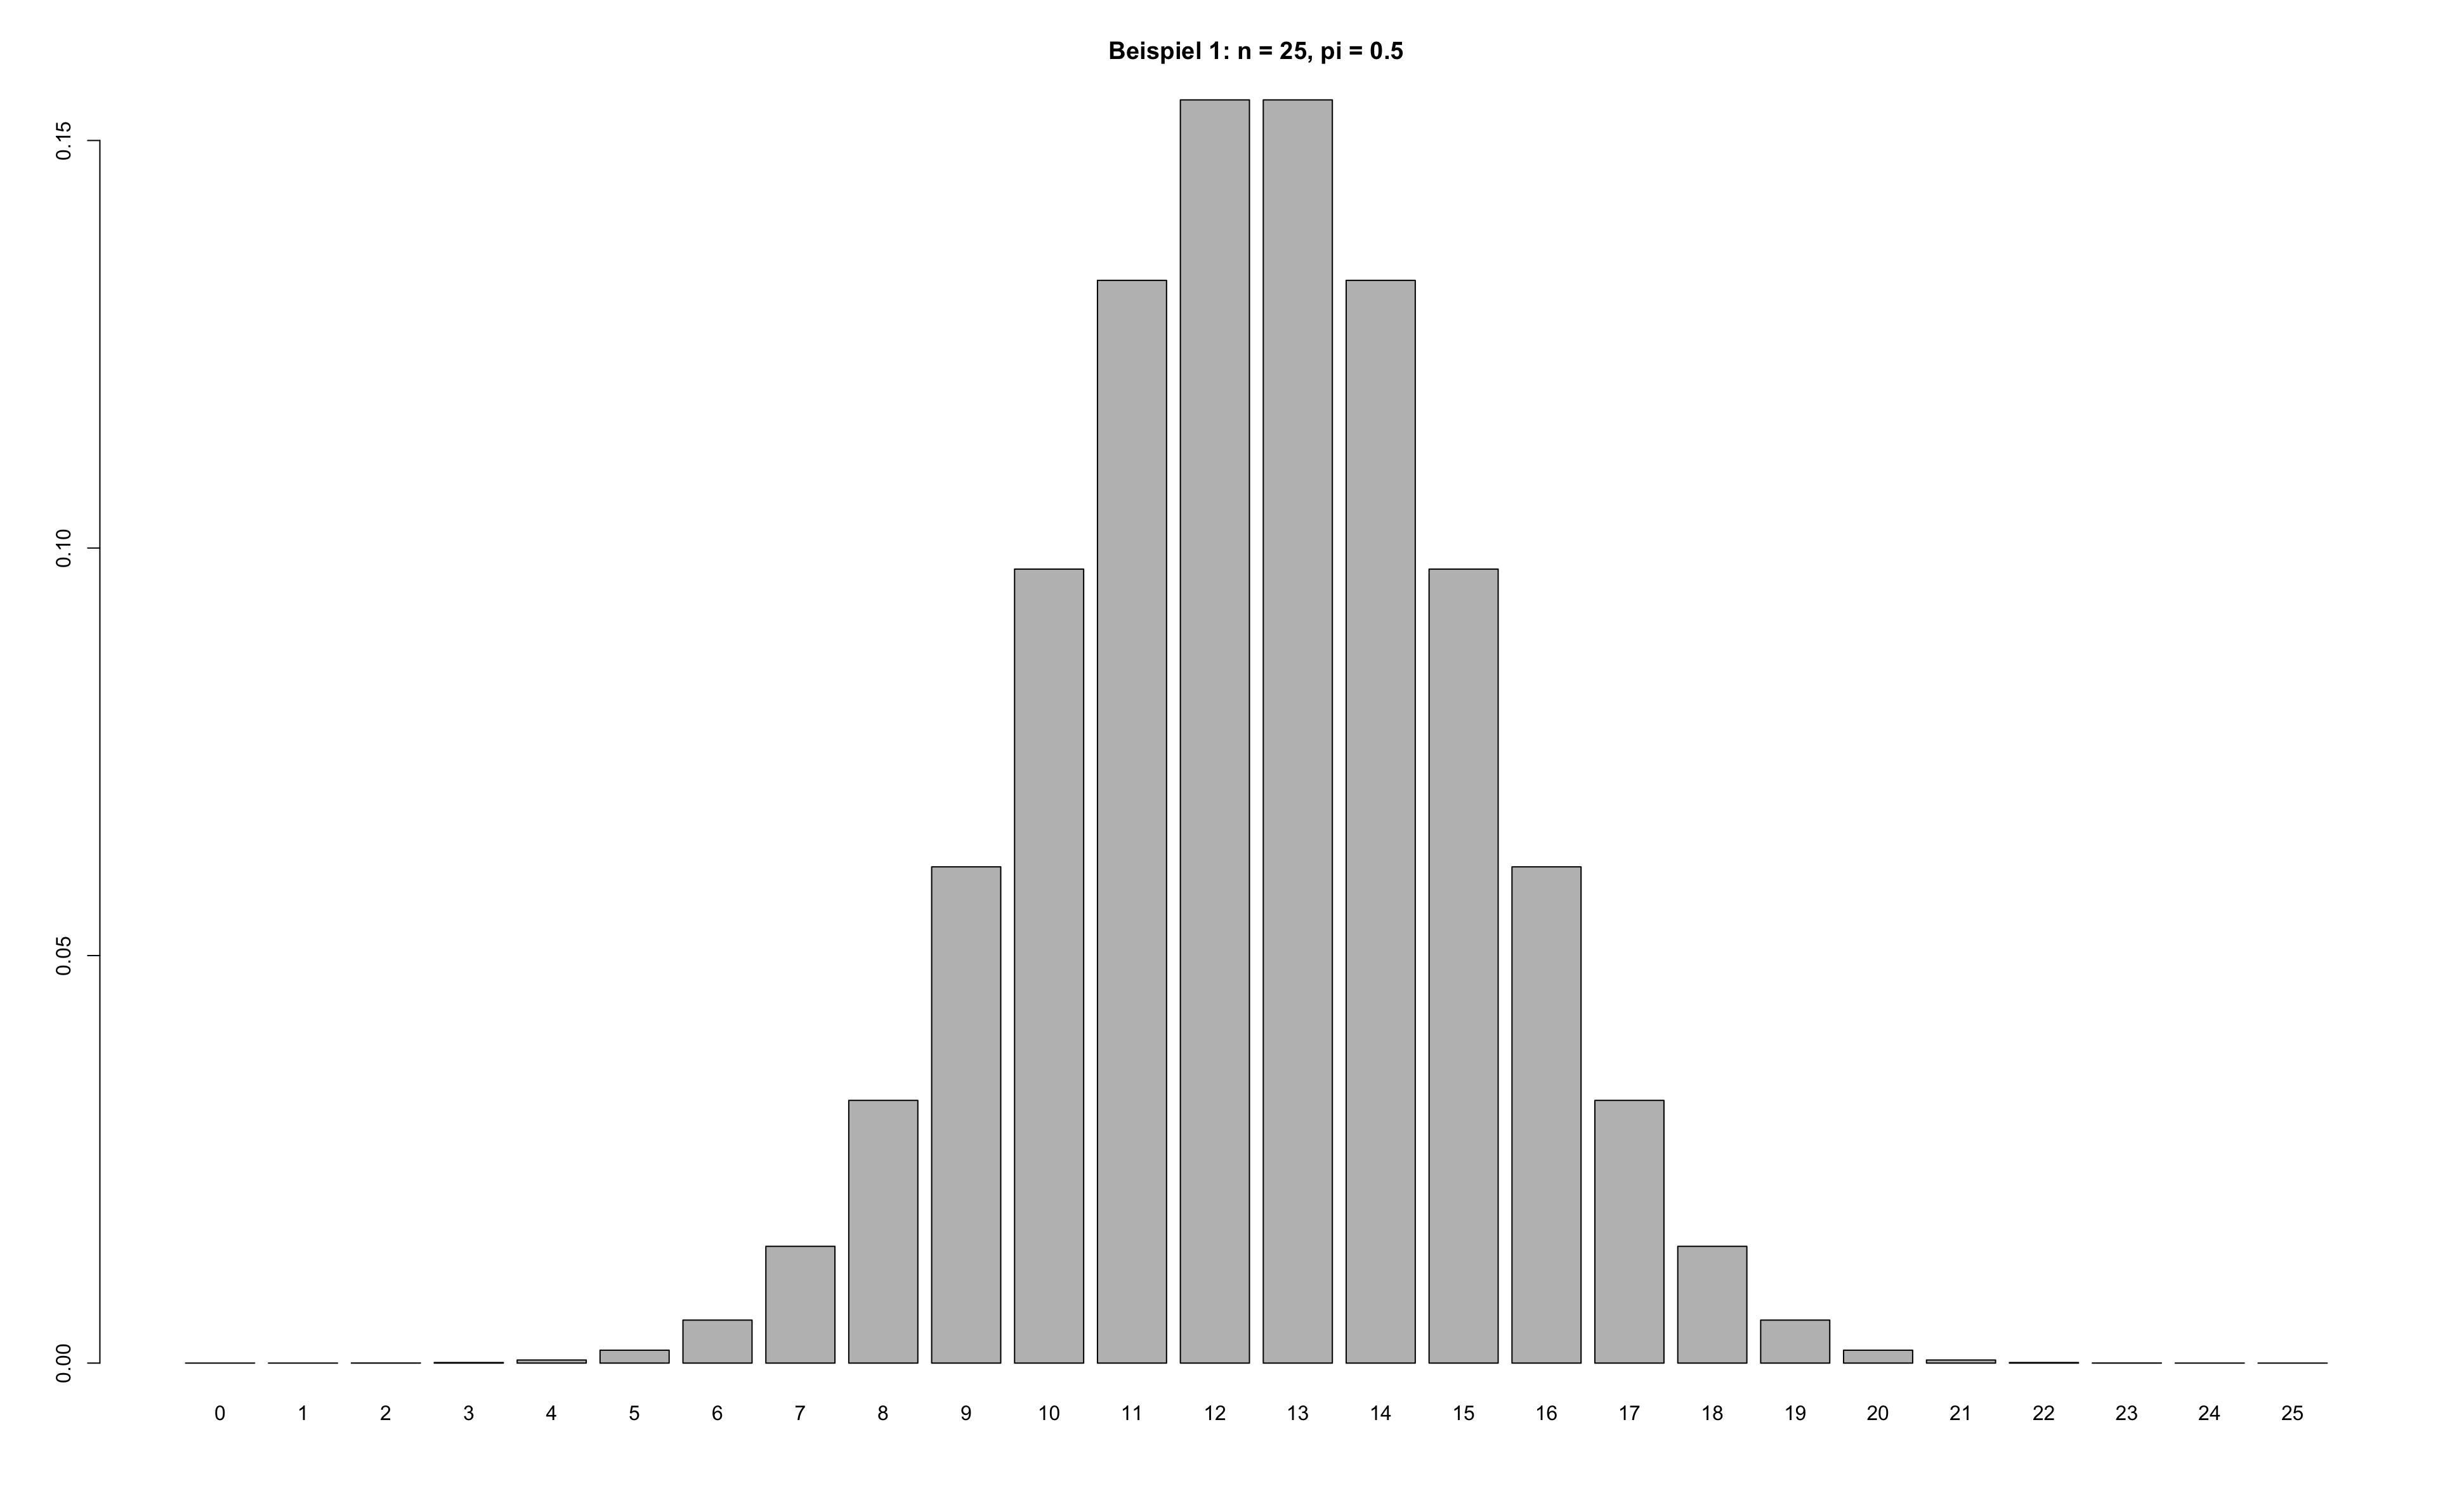
\includegraphics[width=0.45\textwidth]{Rplot02.png}

\vspace{0.8em}

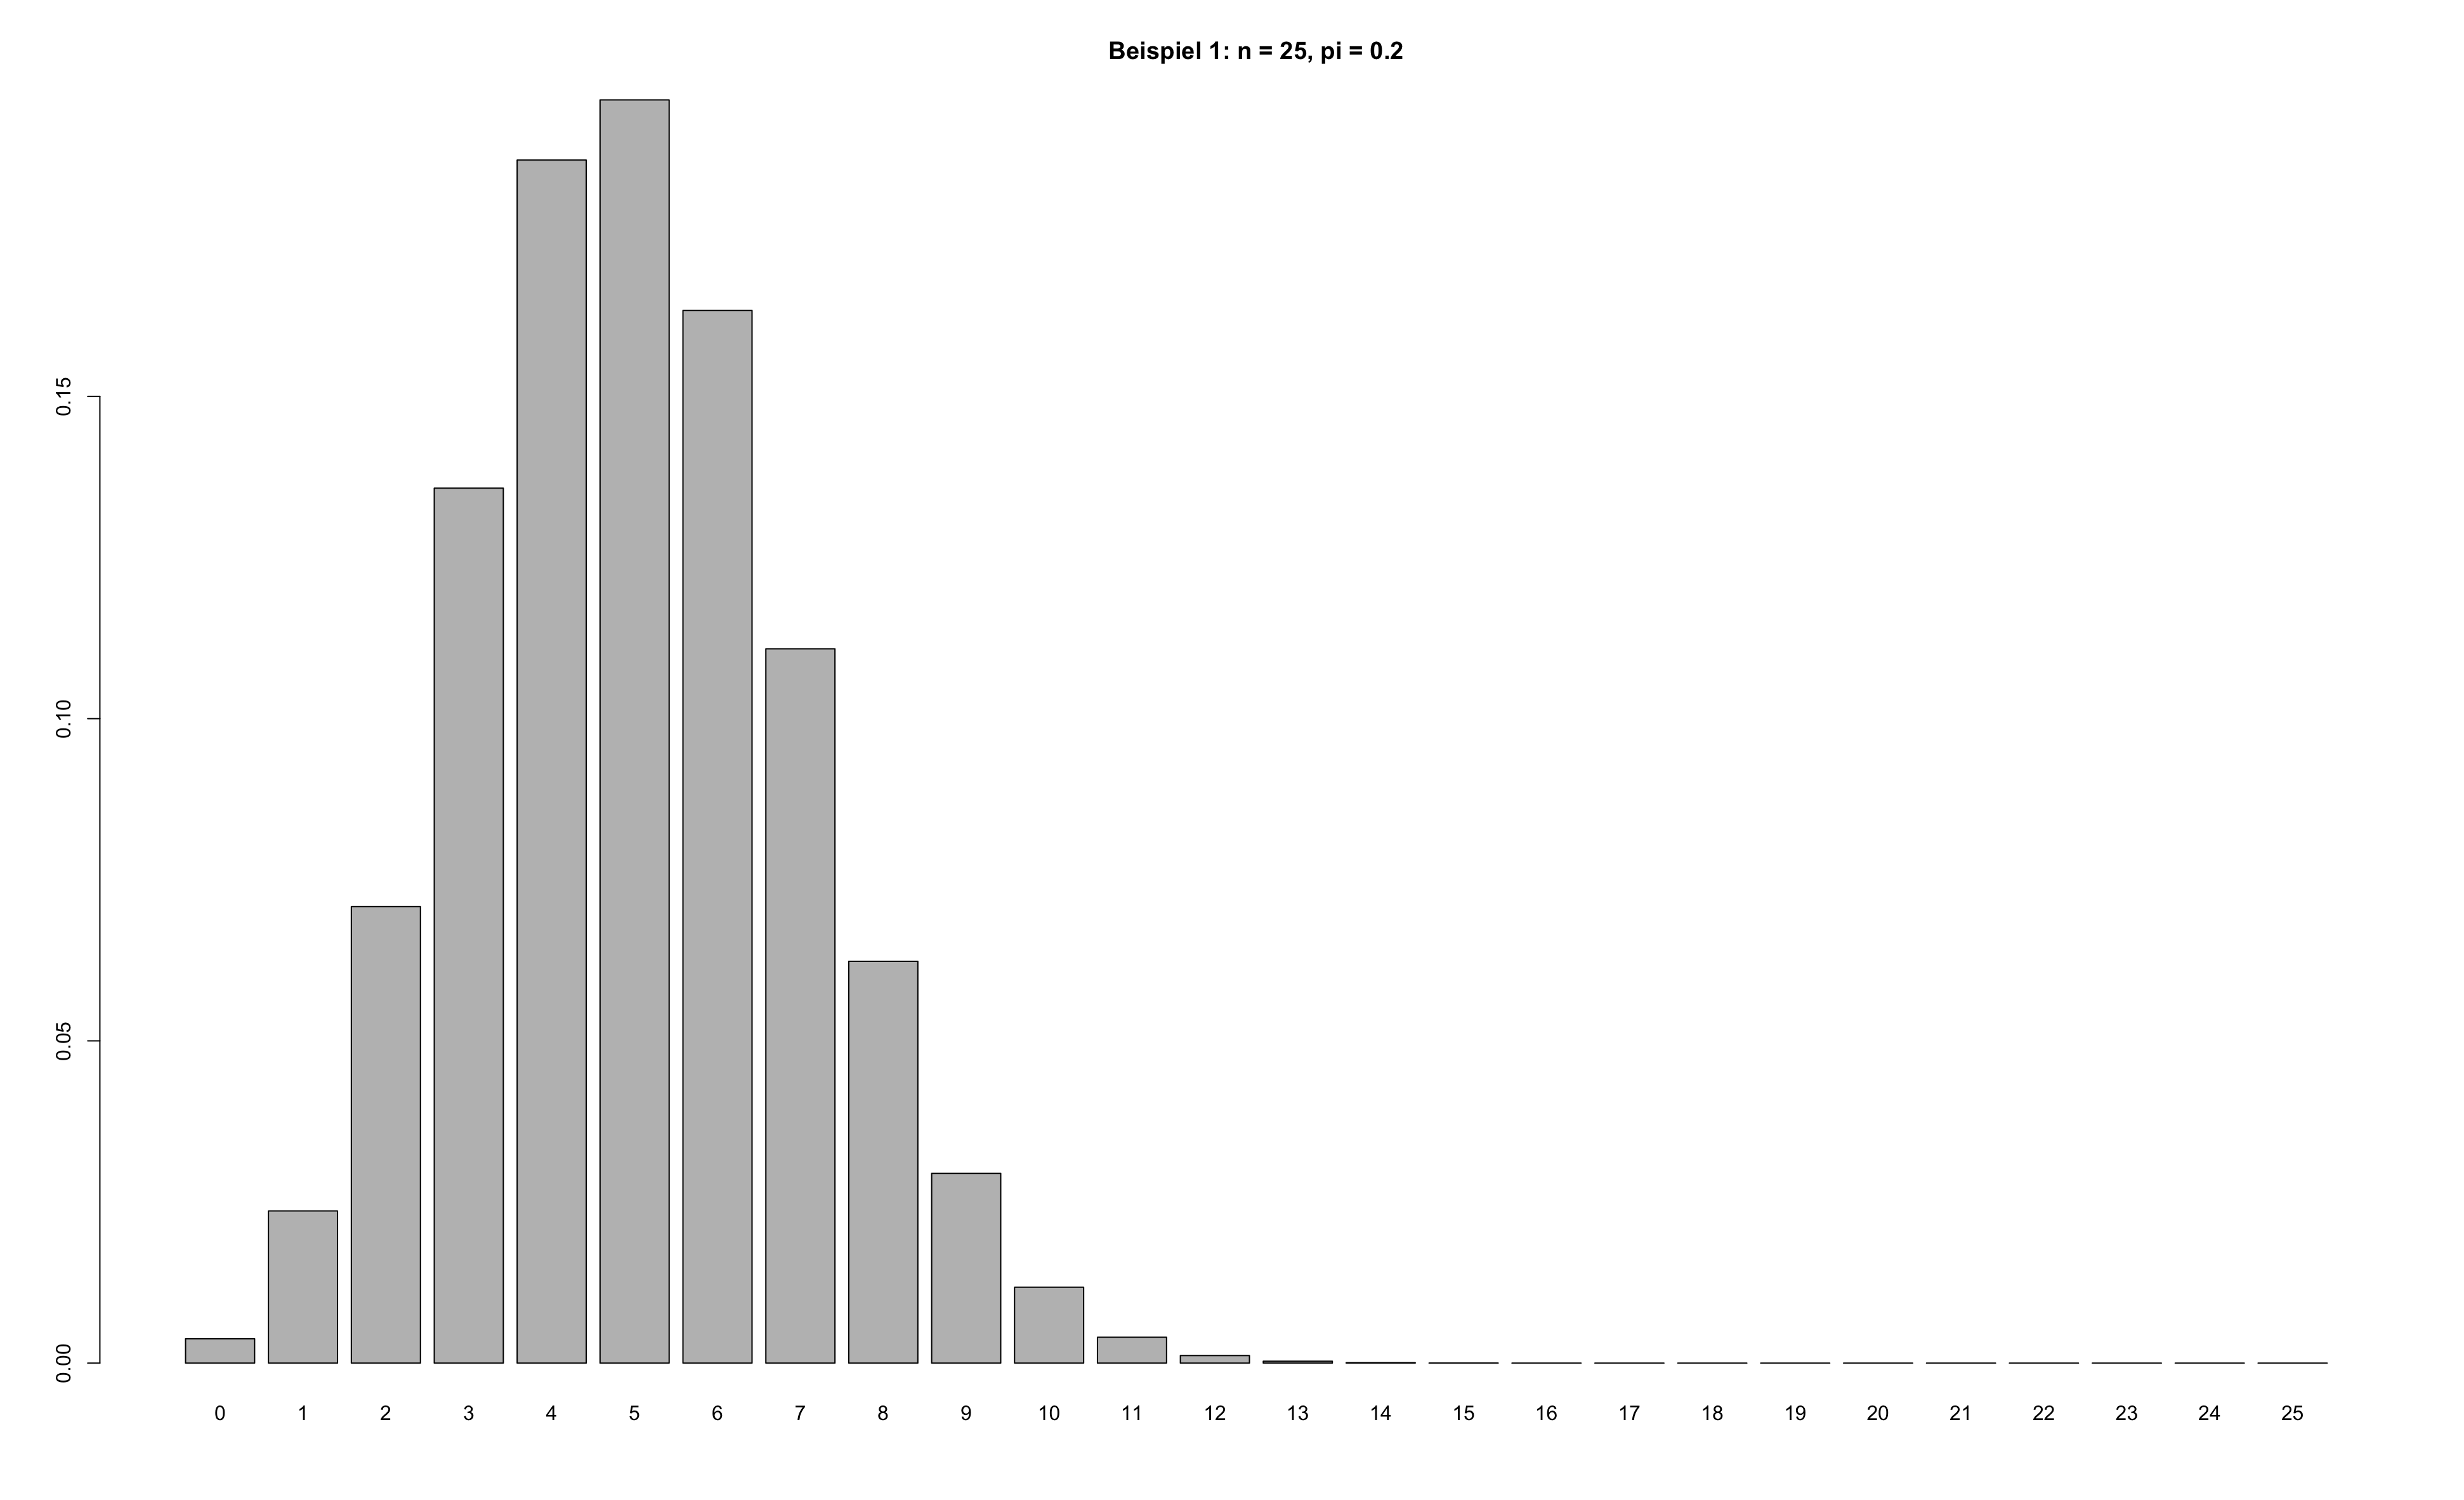
\includegraphics[width=0.45\textwidth]{Rplot01.png}
\hfill
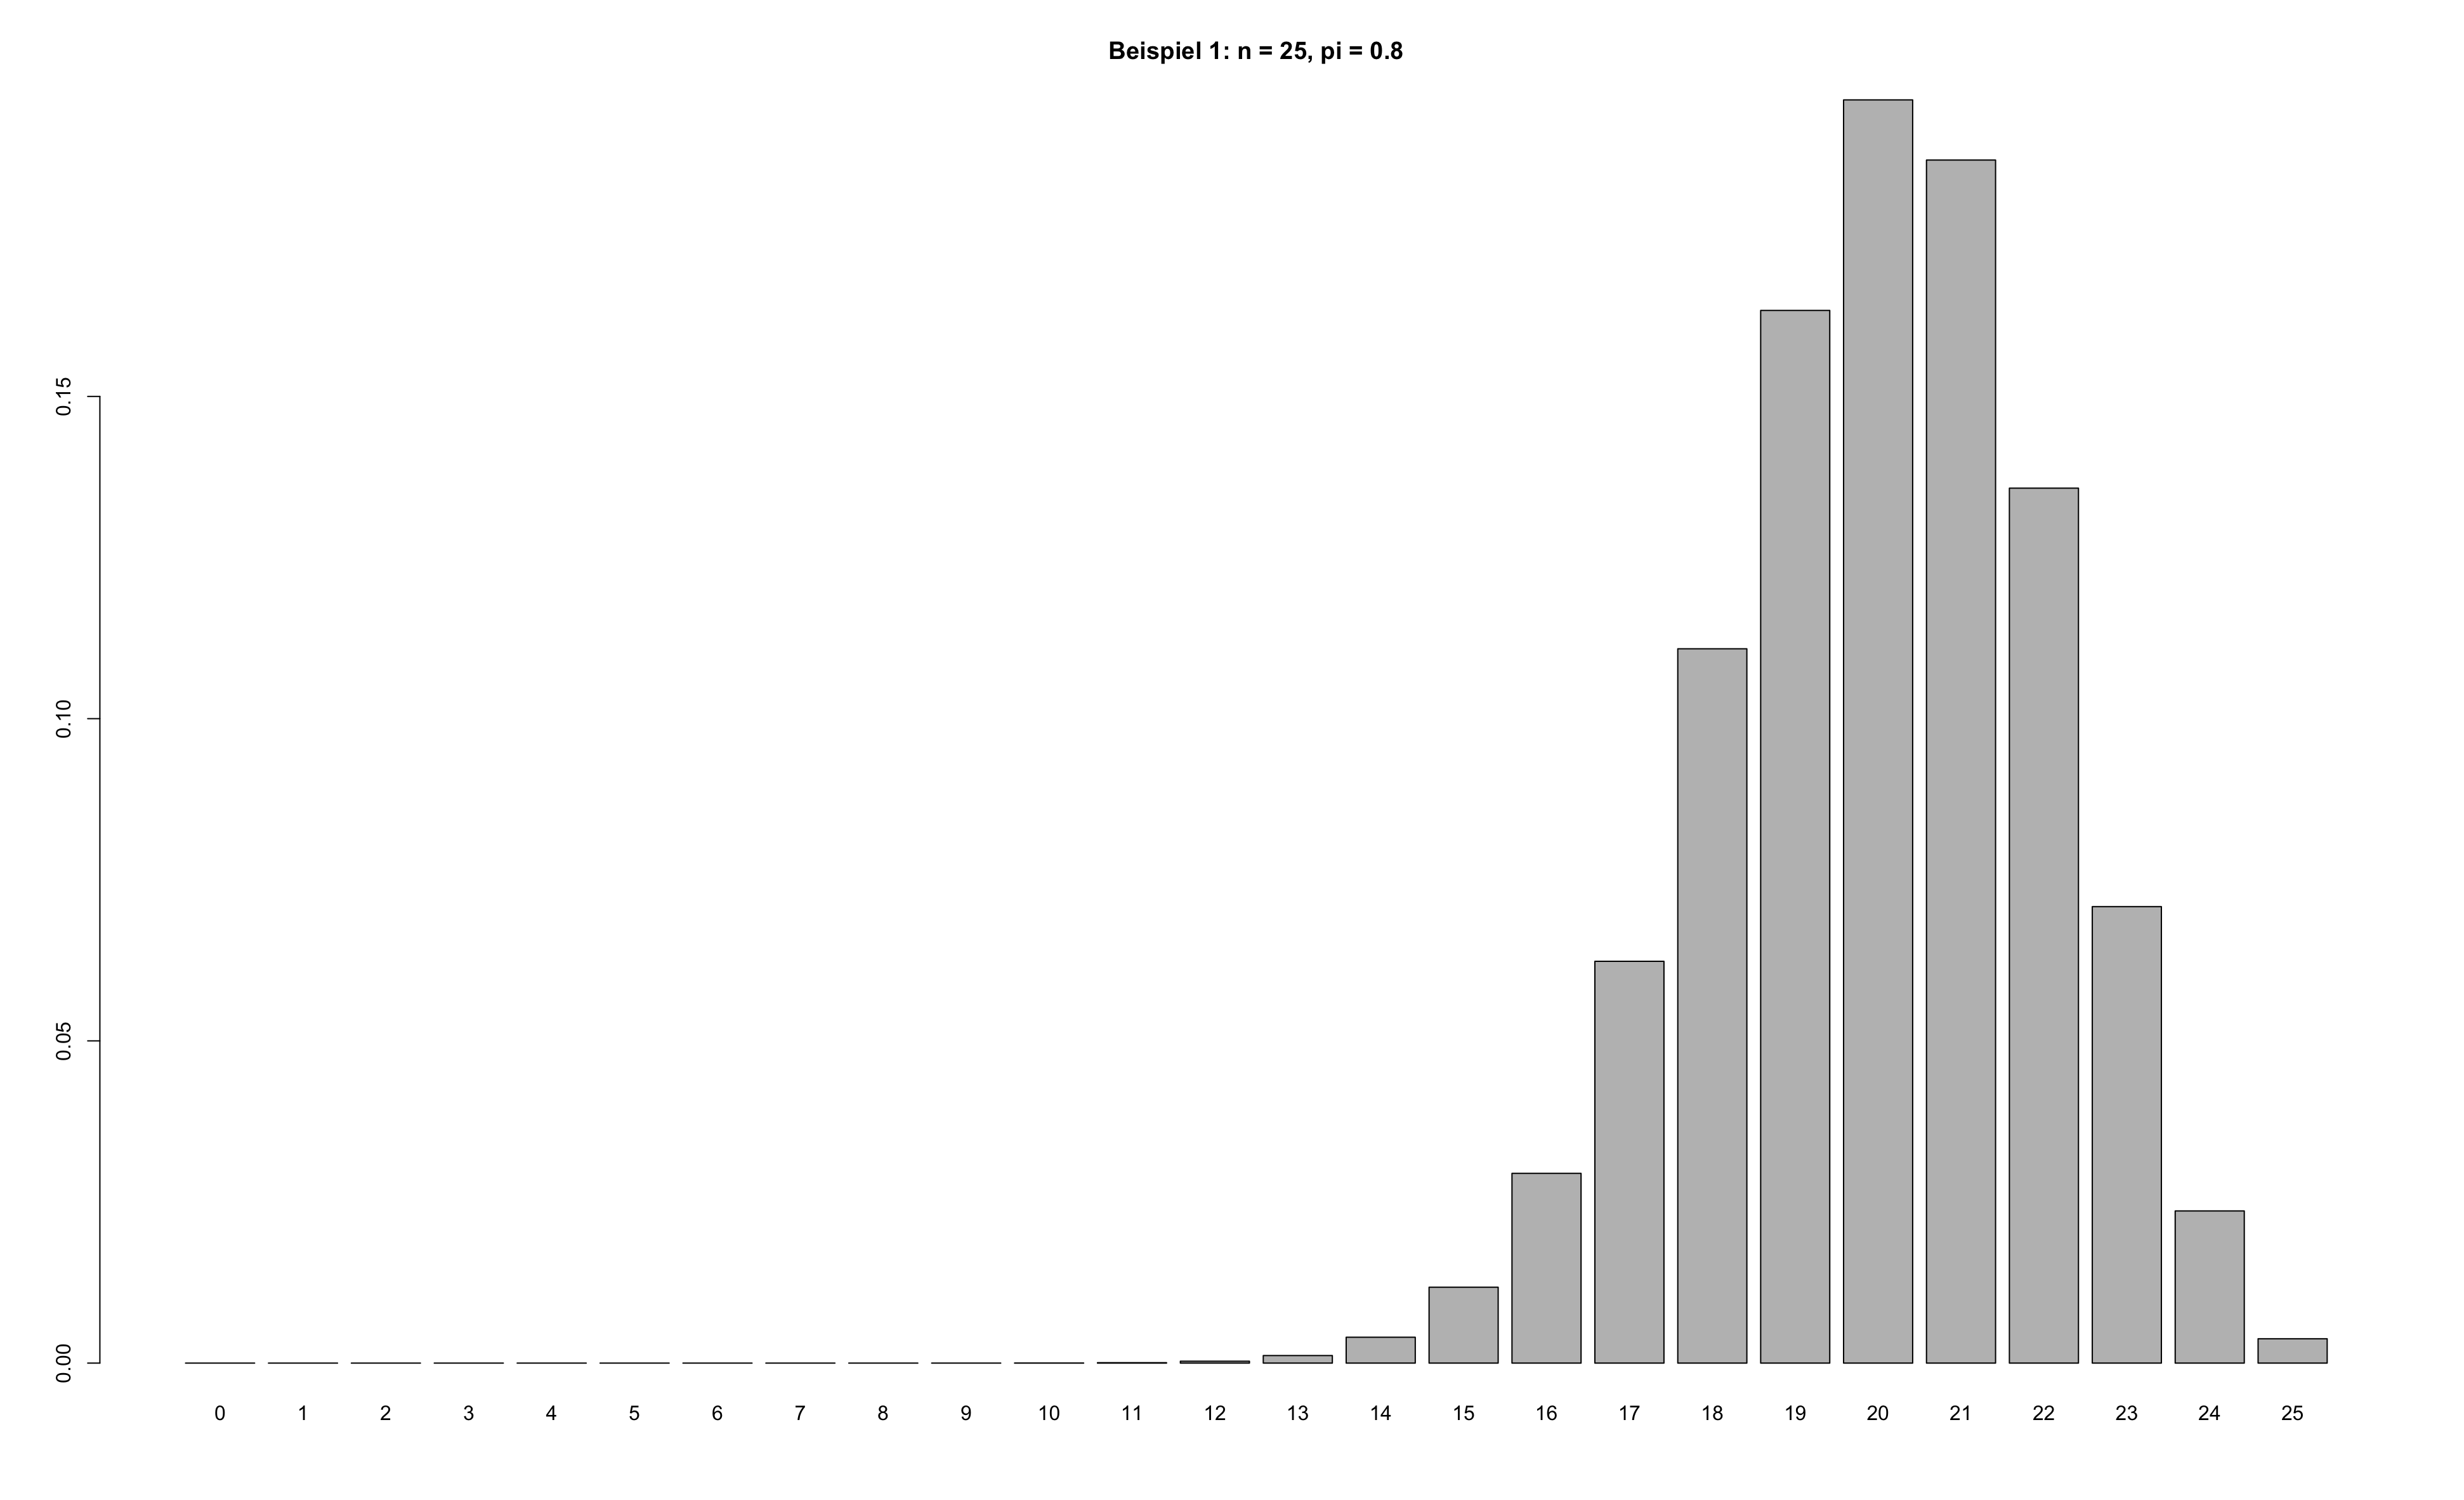
\includegraphics[width=0.45\textwidth]{Rplot03.png}

\caption{Vergleich dreier Binomialverteilungen.}
\end{figure}

Die Abbildung zeigt, dass $(n,\pi)$ bestimmt, wo der Mittelwert (höchste Punkt) der Binomialverteilung ist. Wenn $n=25$ und $\pi=0.25$, dann ist der Mittelwert der Binomialverteilung in $\mu=\mathbb{E}(x)=n\pi=6.25$.

\end{definition}

\subsection{Hypergeometrische Verteilung}
\begin{definition}[Hypergeometrische Verteilung, Stichprobe ohne Zurücklegen]
Für diese Art von Verteilung ergibt sich folgende Wahrscheinlichkeitsfunktion:

\begin{equation}
\mathbb{P}(X=x)=\frac{\begin{pmatrix} s \\ x \end{pmatrix} \begin{pmatrix} N-s \\ n-x \end{pmatrix}}{\begin{pmatrix} N \\ n \end{pmatrix}},
\end{equation}

mit Grundgesamtheit $N$, Stichprobengrösse $n$, Anzahl Erfolge $s$ in der Grundgesamtheit, Anzahl Erfolge $x$ in der Stichprobe.
\end{definition}

\begin{lemma}[Lageparameter einer hypergeometrischen Verteilung]
Der Erwartungswert einer hypergeometrischen Verteilung berechnet sich als $\mu=\mathbb{E}(X)=\frac{ns}{N}$, wobei $s/N$ der Erfolgswahrscheinlichkeit beim ersten Versuch entspricht. Die Varianz entspricht $\sigma^2=\mathbb{E}[(X-\mu)^2]=\frac{ns(N-s)}{N^2}\cdot\frac{(N-n)}{(N-1)}$ mit Korrekturfaktor $\frac{(N-n)}{(N-1)}$.
\end{lemma}

\subsection{Poisson-Verteilung}
\begin{definition}[Poisson-Verteilung]
Eine (diskrete) Zufallsvariable besitzt die Poisson-Verteilung mit dem Parameter $n\pi \textgreater 0$, wenn sie Werte in $\mathbb{N}$ annimmt und für $k\in \mathbb{N}$ die folgende Wahrscheinlichkeitsfunktion aufweist:

\[f_X(x)=\mathbb{P}[X=x]=\frac{e^{-\lambda}\lambda^x}{x!}. \]

Wir schreiben $X \sim \text{Pois}(n\pi)$, um anzugeben, dass $X$ gemäss der Poisson-Verteilung mit dem Parameter $n\pi=\lambda$ verteilt ist. $\mathbb{P}[X=x]$ ist die Wahrscheinlichkeit, dass das Ereignis genau $x$-mal innerhalb eines Zeitraums eintreffen wird. Der Erwartungswert und die Varianz der Poissonverteilung sind genau gleich. Anwendung findet die Poissonverteilung meist dann, wenn $n$ und $\pi$ nicht einzeln bekannt sind, sondern lediglich der Mittelwert $\lambda=n\pi$; und $\pi$ sehr klein ist ($< 0.05$ nach Weiers).

\begin{figure}[ht]
\centering

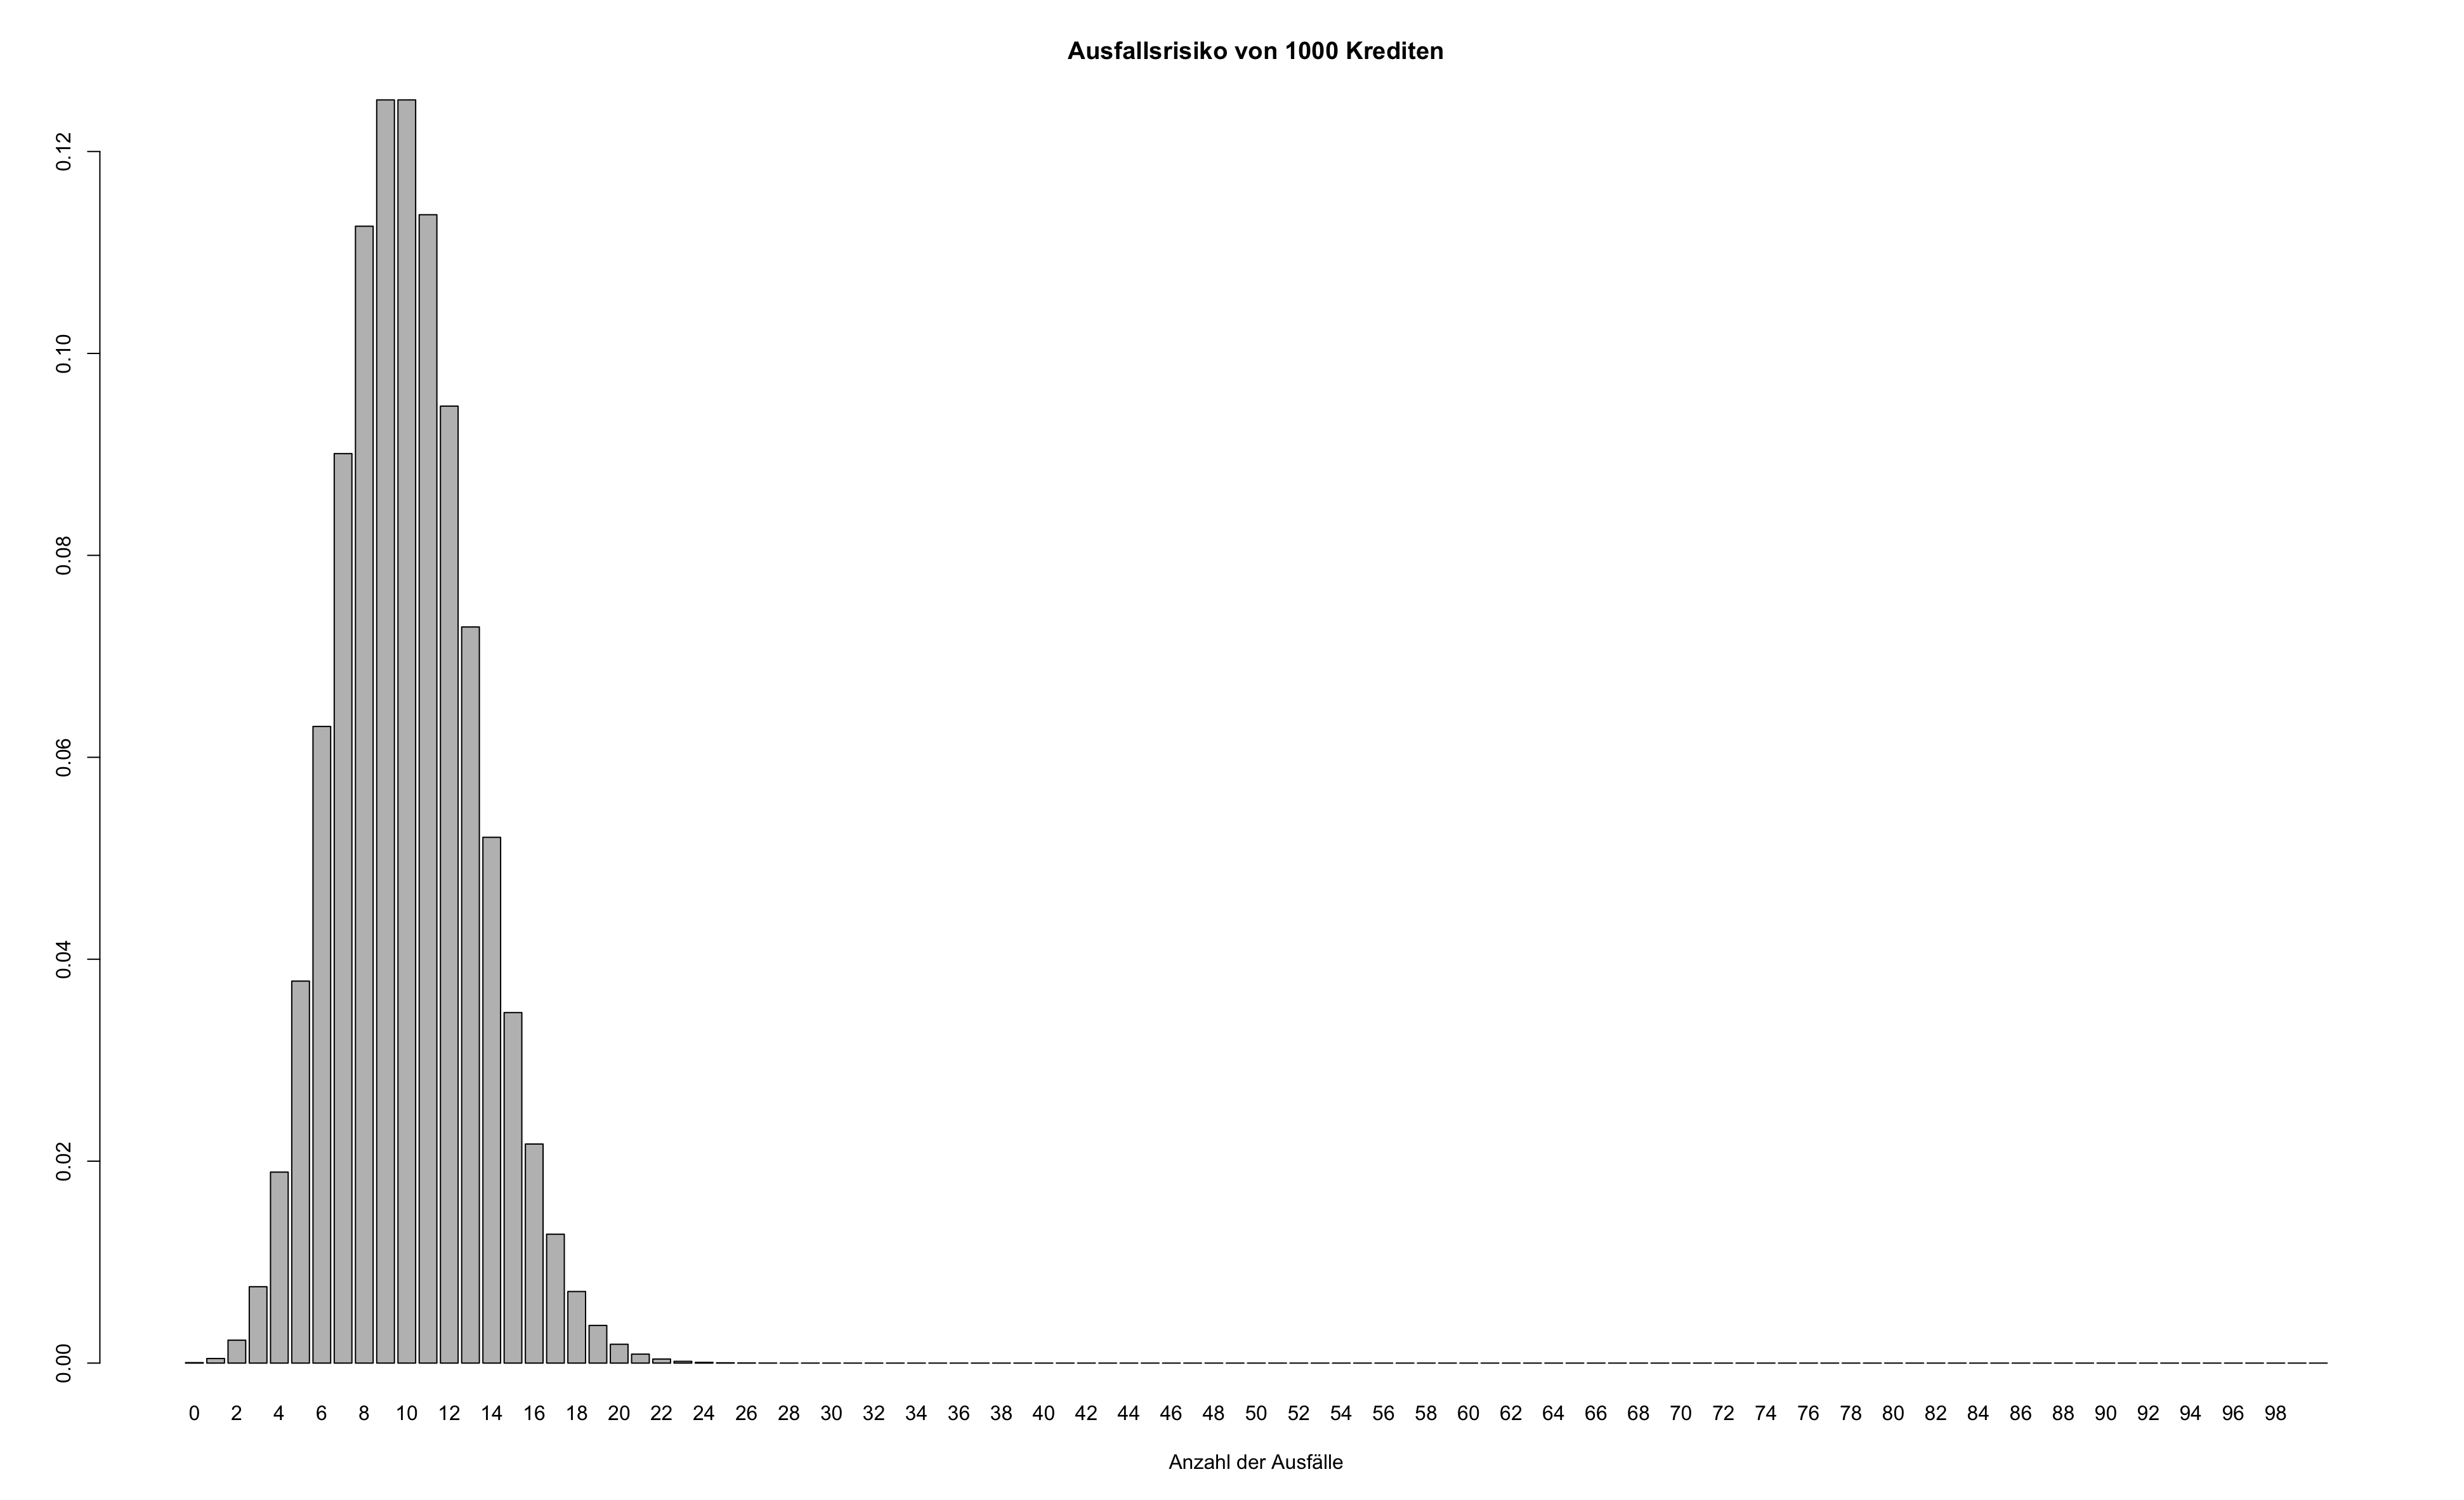
\includegraphics[width=\textwidth]{poisson1.png}

\caption{Ausfallwahrscheinlichkeit der Kredite aus Sicht eines Finanzinstituts mit $p=0.01, n=1000$.}
\end{figure}

Wir sehen, dass bei einem Portfolio von 1000 Krediten die Wahrscheinlichkeit, dass zehn bis zwölf Kredite ausfallen bei ca. $12\%$ liegt. Die Wahrscheinlichkeit eines Ausfalls ist tief und Poisson-verteilt.
\end{definition}

\subsection{Uniform Distribution}
A uniform random variable, typically written \(U[a,b]\), has density
\[ f(x|a,b)=\frac{1}{b-a}, \quad a \leq x \leq b. \]
\[ \mathbb{E}[X]=\frac{b+a}{2} \]
\[ \text{var}[X]=\frac{(b-a)^2}{12} \]

% NEW SECTION

\section{Stetige Verteilungen und Normalverteilung}
\subsection{Lernziele}
Nach dieser Vorlesung hat man gelernt, wie der Erwartungswert und die Varianz im Falle von stetigen Verteilungen berechnet werden ; die Normalverteilung im Bereich der BWL angewendet wird und warum sie dort von zentraler Bedeutung ist; eine Normalverteilung standardisiert wird und wieso die Standardnormalverteilung wichtig ist.

\begin{definition}[Dichtefunktion stetiger Zufallsvariablen]
Bei einer stetigen, bzw. kontinuierlichen Zufallsvariablen tritt an Stelle der Wahrscheinlichkeitsfunktion die sogenannte Dichtefunktion. Die Dichtefunktion $f(x)$ einer stetigen Zufallsvariablen $X$ ist eine stetige Funktion für die gilt:

\[\int_{-\infty}^{\infty} f(x) \,dx=1, f(x)\geq 0. \]

Die Dichtefunktion kann somit nicht negativ werden und die Fläche zwischen der Dichtefunktion und der x-Achse ergibt genau $1$.
\end{definition}

\begin{definition}[Wahrscheinlichkeit eines Ereignisses]
Die Wahrscheinlichkeit, dass $X$ einen Wert im Intervall $[a,b]$ annimmt, entspricht der Fläche unter der Dichtefunktion in den Grenzen $a$ und $b$. Wir schreiben $\mathbb{P}(a\leq X \leq b)=\int_{a}^{b} f(x) \,dx=F(b)-F(a).$
\end{definition}

\begin{definition}[Kumulierte Verteilungsfunktion]
Die Kumulierte Verteilungsfunktion gibt uns die Wahrscheinlichkeit, dass ein Elementarereignis realisiert wird, das höchstens den Wert $a$ annimmt: $F(a)=\mathbb{P}(X\leq a)=\int_{-\infty}^{a} f(x) \, dx.$
\end{definition}

\begin{definition}[Erwartungswert einer Dichtefunktion]
Der Erwartungswert einer Dichtefunktion errechnet sich als $\mathbb{E}(X)=\int_{-\infty}^{\infty}xf(x) \, dx.$
\end{definition}

\begin{definition}[Varianz einer Dichtefunktion]
Die Varianz einer Dichtefunktion errechnet sich als $\mathbb{E}(X^2)-[ \mathbb{E}(X)]^2$
\end{definition}

\begin{definition}[Normalverteilung]
Eine stetige Zufallsvariable mit der Dichtefunktion

\[ f(x)=\frac{1}{\sigma \sqrt{2\pi}}e^{-\frac{1}{2}\left(\frac{x-\mu}{\sigma}\right)^2} \]

ist normalverteilt mit den Parametern $\mu$ und $\sigma^2$. Unter anderen kann auch die Binomialverteilung durch die Normalverteilung approximiert werden. Wir schreiben die Normalverteilung als $N(\mu,\sigma^2)$
\end{definition}

\begin{definition}[Standardnormalverteilung]
Die Standardnormalverteilung ergibt sich bei $\mu=0, \sigma^2=1$ und schreibt sich als $N(0,1)$. Wir berechnen folgende funktionen für die Standardnormalverteilung und deren kumulierte Verteilungsfunktion

\[ \text{Standardnormalverteilung:} \qquad f(x)=\frac{1}{\sqrt{2\pi}}e^{-\frac{x^2}{2}} \]
\[ \text{Standardnormalverteilung CDF:} \qquad \Phi(z)=\int_{-\infty}^{z}\frac{1}{\sqrt{2\pi}}e^{-\frac{x^2}{2}} \, dx\]

\end{definition}

\begin{theorem}[Zentraler Grenzwertsatz]
Der Zentrale Grenzwertsatz besagt, dass Stichprobenmittelwerte sowie Anteilswerte von wiederholten Stichproben zu einer Normalverteilung tendieren.
\end{theorem}

% NEW SECTION

\section{Mehrdimensionale Verteilungen}
\subsection{Lernziele}
Nach dieser Vorlesung hat man gelernt, wie die Wahrscheinlichkeitskonzepte für zweidimensionale Zufallsvariablen angewendet werden; konkrete Fragestellungen anhand der 4-Felder-Tafel gelöst werden; die Konzepte der Kovarianz und Korrelation auf Zufallsvariablen angewandt werden; stochastische Unabhängigkeit zwischen zwei Zufallsvariablen bestimmt wird. 

\vspace{1em}

\begin{definition}[Gemeinsame Wahrscheinlichkeitsfunktion]
Die gemeinsame Wahrscheinlichkeitsfunktion \(f(x_i,y_k)\) gibt die Wahrscheinlichkeit an, dass \(X\) den Wert \(x_i\) und \(Y\) den  Wert \(y_k\) annimmt. \(X,Y\) sind dabei diskrete Zufallsvariablen mit Realisierungen \(x_1,x_2,..\) und \(y_1,y_2,..\). Wir stellen fest, dass folgende Eigenschaften gelten:

\[ f(x_i,y_k)=P(X=x_i,Y=y_k) \]
\[ f(x_i,y_k) \geq 0\]
\[ \sum_{i}\sum_{k}f(x_i,y_k)=1. \]

Dies ist eine Doppelsumme, wobei wir die innere von der äusseren Summe unterscheiden. Sei \(i=\{1,2,3\}, n=\{1,2,3\}\). Die Innere Summe ist folglich

\[ \sum_{k}f(x_i,y_k)= f(x_i,y_1)+f(x_i,y_2)+f(x_i,y_3), \]
 
woraus die äussere Summe entsteht:

\[ \sum_{i}\left[f(x_i,y_1)+f(x_i,y_2)+f(x_i,y_3)\right] \]
\[ \Leftrightarrow f(x_1,y_1)+f(x_1,y_2)+f(x_1,y_3)+f(x_2,y_1)+f(x_2,y_2)+f(x_2,y_3)+f(x_3,y_1)+f(x_3,y_2)+f(x_3,y_3) \]

 
\end{definition}

\begin{definition}[Gemeinsame Verteilungsfunktion]
Die gemeinsame Verteilungsfunktion \(F(x,y)\) gibt die Wahrscheinlichkeit an, dass \(X\) höchstens den Wert \(x\) und gleichzeitig \(Y\) höchstens den Wert \(y\) annimt. \(X,Y\) sind dabei wieder diskrete Zufallsvariablen. Wir scheiben
\[ F(x,y)=P(X=X\leq x,Y\leq y) \]
\[ F(x,y)\sum_{x_i\leq x}\sum_{y_k\leq y}f(x_i,y_k). \]
Zudem gilt folgendes für Randverteilungen
\[ f_X(x_i)=P(X=x_i)=\sum_{k}f(x_i,y_k), \]
\[ f_Y(y_k)=P(Y=y_k)=\sum_{i}f(x_i,y_k). \]
\end{definition}

\begin{definition}[Bedingte Verteilungen]
Die bedingte Verteilung von \(X\) gegeben \(Y\) is definiert durch
\[f(x_i|y_k)=\frac{f(x_i,y_k)}{f_Y(y_k)}\]
\end{definition}

\begin{definition}[Bedingter Erwartungswert und Varianz]
Die Bedingten Erwartungswerte lassen sich über die bedingten Wahrscheinlichkeiten bestimmen
\[ \mathbb{E}[X|Y]=\sum_{i=1}^{n}x_if(x_i|Y)\]
Darauf aufbauen leiten wir die Formel für die Bedingte Varianz her
\[ \text{Var}(X|Y)=\sum_{i=1}^{n}x_i^2f(x_i|Y)-\left[\mathbb{E}[X|Y]\right]^2\]
\end{definition}

\begin{definition}[Kovarianz und Korrelationskoeffizient]
Kovarianz und Korrelationskoeffizien sind Masse für die Stärke eines statistischen Zusammenhangs zweier metrisch messbaren Merkmale. Der Korrelationskoeffizient \(\rho\) nimmt immer einen Wert in \((-1,1)\) ein. Im allgemeinen lässt sich sagen, dass ein Korrelation ungleich null immer impliziert, dass Ereignisse abhängig sind, jedoch lässt sich mit einem Korrelationskoeffizient von null nicht bestimmt sagen, dass die Ereignisse abhängig sind. Es gelten folgende Formeln
\[ Cov(X,Y)=\mathbb{E}[XY]-\mathbb{E}[X]\mathbb{E}[Y]\]
\[Corr(X,Y)=\rho(X,Y)=\frac{cov(X,Y)}{\sqrt{var[X]var[Y]}}.\]
\end{definition}

\section{Stichprobenverteilungen}
\subsection{Lernziele}
Nach dieser Vorlesung hat man gelernt, wie Stichprobe und Grundgesamtheit unterschieden werden; der zentrale Grenzwertsatz unser Vorgehen beeinflusst; die Stichprobenverteilung für den Mittelwert und den Anteilswert aussieht.

\vspace{1em}

Die Umwandlung in Standardnormalverteilung erfolgt gemäss dieser Formel

\[ z=\frac{\overline{x}-\mu}{\sigma_{\overline{x}}} =\frac{\overline{x}-\mu}{\sigma/\sqrt{n}}, \]
wobei \(\sigma/\sqrt{n}\) der Standardfehler des Stichprobenmittelwerts \(\sigma_{\overline{x}}\) ist.

\begin{definition}[Zentraler Grenzwertsatz]
Die Verteilung des arithmetischen Mittelwerts von \(n\) i.i.d. Zufallsvariablen \(X_i\) strebt mit wachsendem Stichprobenumfang \(n\) gegen eine Normalverteilung mit dem Erwartungswert \(\mu\) und der Varianz \(\sigma^2/n\) (asymptotisch normalverteilt). Als Folge rechtfertigt der zentrale Grenzwertsatz, dass für jede Verteilung der zugrundeliegenden Grundgesamtheit die Verteilung des Mittelwertes durch die Normalverteilung angenähert werden kann, solange die Stichprobengrösse ausreichen gross ist \(n\geq30\).

\begin{figure}[ht]
\centering

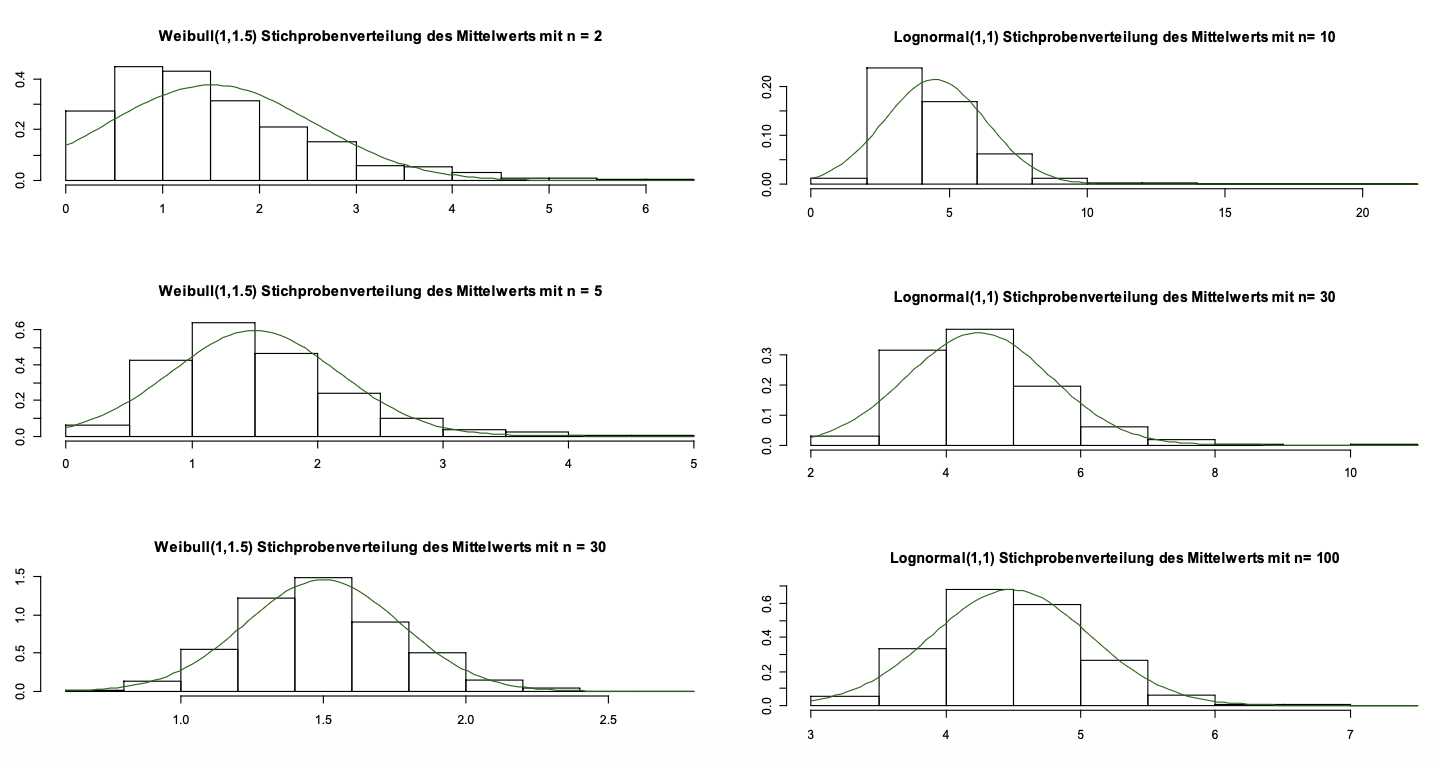
\includegraphics[width=\textwidth]{zentraler_grenzwertsatz.png}

\caption{Der Zentrale Grenzwertsatz in Aktion bei einer Weibull- und Lognormal-Verteilung.}
\end{figure}

\end{definition}

% Stichprobenanteilswert und Beispiel

\section{Schätztheorie}
\subsection{Lernziele}
Nach dieser Vorlesung hat man gelernt, wie die Grundbegriffe der Schätztheorie und die erforderlichen Eigenschaften von Schätzungen lauten; Stichprobenstatistiken sich von den entsprechenden Werten der Grundgesamtheit unterscheiden; man Konfidenzintervalle für Mittel- und Anteilswerte bildet und wann die t-Verteilung bei Konfidenzintervallen angewandt werden soll; gross der erforderliche Stichprobenumfang sein soll.

\vspace{1em}

\begin{definition}[Konfidenzintervall]
Eine Zufallsvariable \(\overline{X}\) ist unter den Annahmen einer normalverteilten Grundgesamtheit und einem genügend grossem Stichprobenumfang normalverteilt mit
\[ \mathbb{E}=\mu, \quad \text{Var}(\overline{X})=\sigma_{\overline{X}}^2=\frac{\sigma^2}{n},\]
\[ \frac{\overline{X}-\mu}{\sigma_{\overline{X}}} \sim N(0,1),\]
\[\mathbb{P}\left[\-z_{a/2}\leq\frac{\overline{X}-\mu}{\sigma_{\overline{X}}}\leq z_{a/2}\right]=1-\alpha,\]
wobei \(z_{a/2}\) der z-Wert ist, welcher \(\alpha/2\) Prozent der Standardnormalverteilung abschneidet.

\begin{figure}[ht]
	\centering
	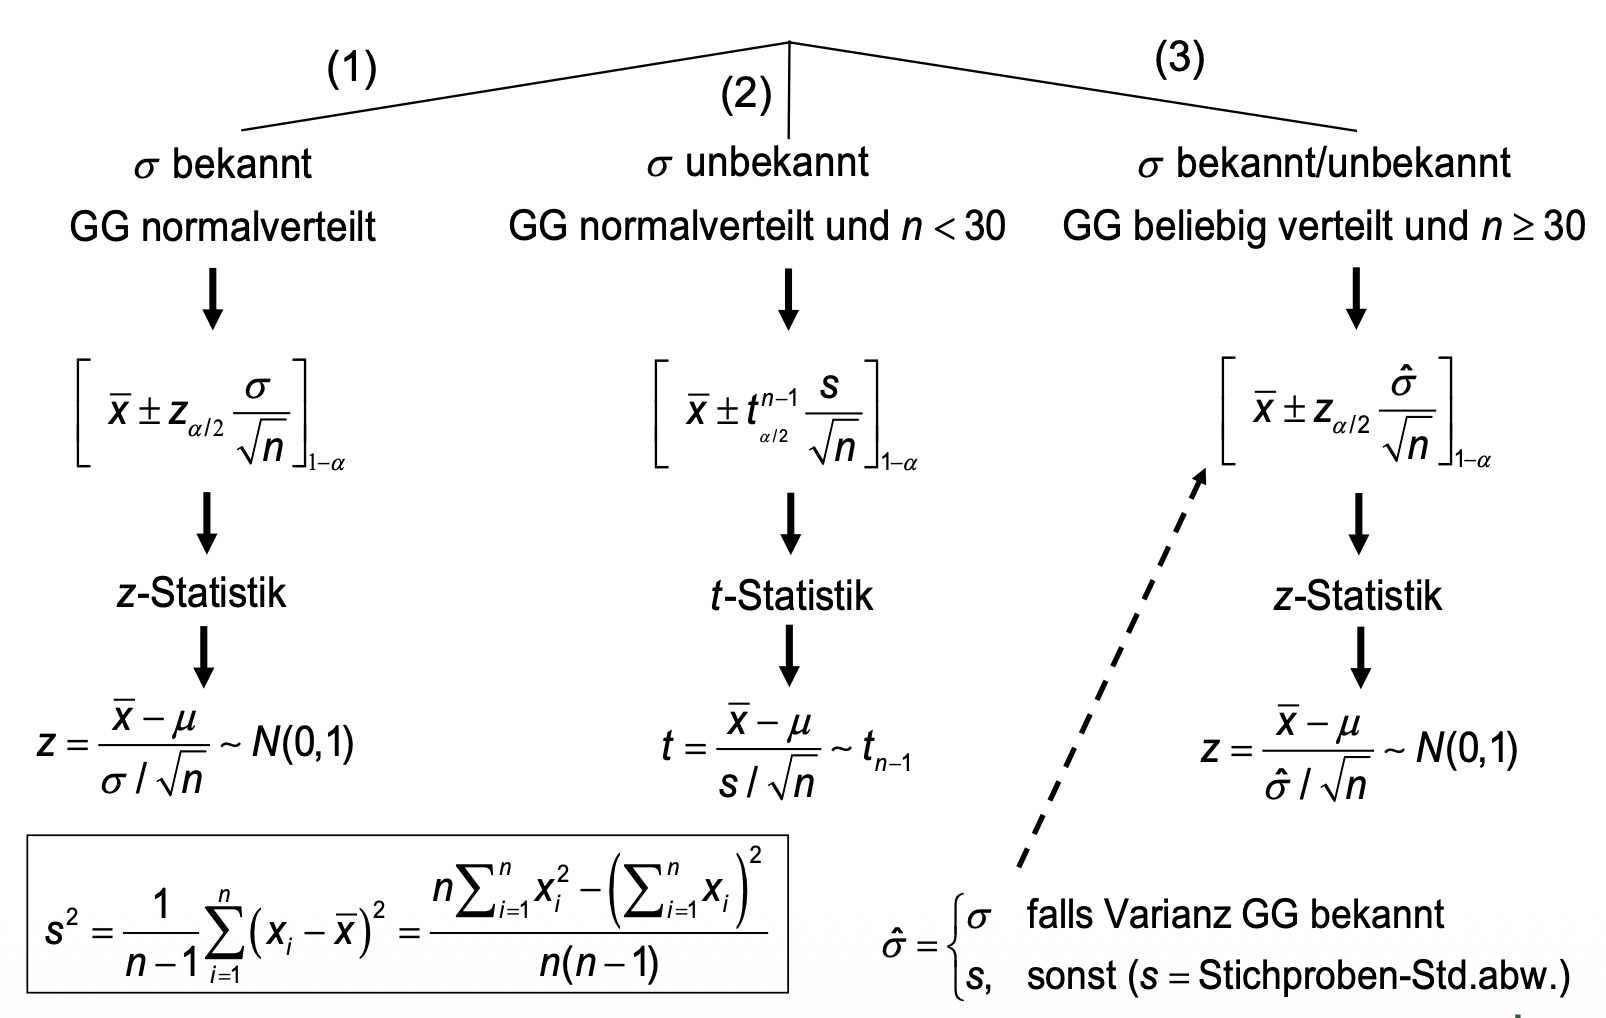
\includegraphics[width=\textwidth]{konfidenzintervalle_des_mittelwerts.png}
		\caption{Konfidenzintervalle des Mittelwerts.}
\end{figure}
\end{definition}

% Konfidenzintervall für den Anteilswert
% Stichprobenumfang

\section{Testtheorie und Hypothesentests}
\subsection{Lernziele}
Nach dieser Vorlesung hat man gelernt, wie Hypothesentests aufgebaut sind und Null- und Alternativhypothese sich im ein- und zweiseitigen Fall unterscheiden; sich Hypothesentests und Intervalleinschätzungen unterscheiden; sich der kritische Wert und der \(\rho\)-Wert als Entscheidungskriterium bei Hypothesentests unterscheiden; sich Fehler der ersten und zweiten Art unterscheiden.

\vspace{1em}

\subsection{Null- und Alternativhypothese}
Wir unterscheiden zwischen zweiseitigen Hypothesen, (einseitigen) linksseitigen und (einseitigen) rechtsseitigen Hypothesen. Stell dir eine Normalverteilung um null vor. Bei der nicht-direktionalen Hypothese (zweiseitig) wird die Nullhypothese nicht verworfen, wenn \(|t|>z_{\alpha/2}\). Das heisst alles was innerhalb der Grenzen ist, wird akzeptiert. Bei der direktionalen Hypothese wird die Nullhypothese nicht verworfen, wenn \(t<-t_\alpha\) (linksseitig), bzw. \(t>t_\alpha\) (rechtsseitig).

\vspace{1em}

Hypothesentests werden in folgenden fünf Schritten durchgeführt: Aufstellung der Null- und Alternativhypothese sowie Festlegung des Signifikanzniveaus; Wahl einer geeigneten Prüfgrösse und Testverteilung unter Gültigkeit der Nullhypothese; Bestimmung der kritischen Bereichs; Berechnung der Prüfgrösse; Entscheidung und Interpretation.

\begin{definition}[Fehler 1. und 2. Art]
Der Fehler 1. Art tritt ein, wenn die Nullhypothese \(H_0\) wahr ist und verworfen ist. Analog dazu handelt es sich um einen Fehler 2. Art, wenn \(H_0\) falsch ist und nicht verworfen wird. Das Signifikanzniveau \(\alpha\) gibt die Wahrscheinlichkeit eines Fehlers 1. Art an, während \(\beta\) die Wahrscheinlichkeit eines Fehlers 2. Art widerspiegelt. Bei der Durchführung von Hypothesentests gibt es einen Trade-Off zwischen der Wahrscheinlichkeit beider Fehler.
\end{definition}

% p-Wert

\section{Zweistichprobenverfahren}
\subsection{Lernziele}
Nach dieser Vorlesung hat man gelernt, wie Hypothesentests angewendet werden, um Mittelwerte und Anteilswerte zweier Stichproben zu vergleichen; Konfidenzintervalle um die Differenz zweier Stichprobenmittel- oder -anteilswerte gebildet und interpretiert werden; ein F-Test für den Vergleich zweier Varianzen angewandt und interpretiert wird.

\vspace{1em}

\section{Lineare Regression}
\subsection{Lernziele}
Nach dieser Vorlesung hat man gelernt, wie die lineare Regressionsanalyse aufgebaut ist und welche Bedingungen gelten müssen; Zusammenhänge in einem Datensatz mittels der Regressionsanalyse untersucht und interpretiert werden können.

\vspace{1em}

Wir nennen die unabhängige Variable \(x_k\) einen Regressor und die anhängige Variable \(y\) einen Regressand. Es heisst simple Regression, wenn \(K=1\) und multiple Regression, wenn \(K>1\), d.h. es hängt davon ab, wie viele unabhängige Variablen involviert sind.

\begin{definition}[Bestimmtheitsmass \(R^2\)]
Das Bestimmtheitsmass \(R^2\) gibt an, wieviel Prozent der Varianz der abhängigen Variable vom Modell erklärt wird. Dieses Gütemass nimmt nur Werte in \([0,1]\) an. Es gibt sich folgende Formel
\[ R^2=\frac{SSR}{SST},\]
wobei SSR für Sum of Squares due to Regression und SST für Total Sum of Squares steht. Das Bestimmtheitsmass \(R^2\) lässt sich als Anteil der durch die Regression erklärten Streuung der abhängigen Variable interpretieren. Das bedeutet, dass z.B. ein \(R^2=0.37\) bedeutet, dass 37\% der Streuung in der betrachteten Statistik durch die lineare Abhängigkeit der abhängigen Variable von der erklärenden Variable erklärt werden können.

\begin{figure}[ht]
	\centering
	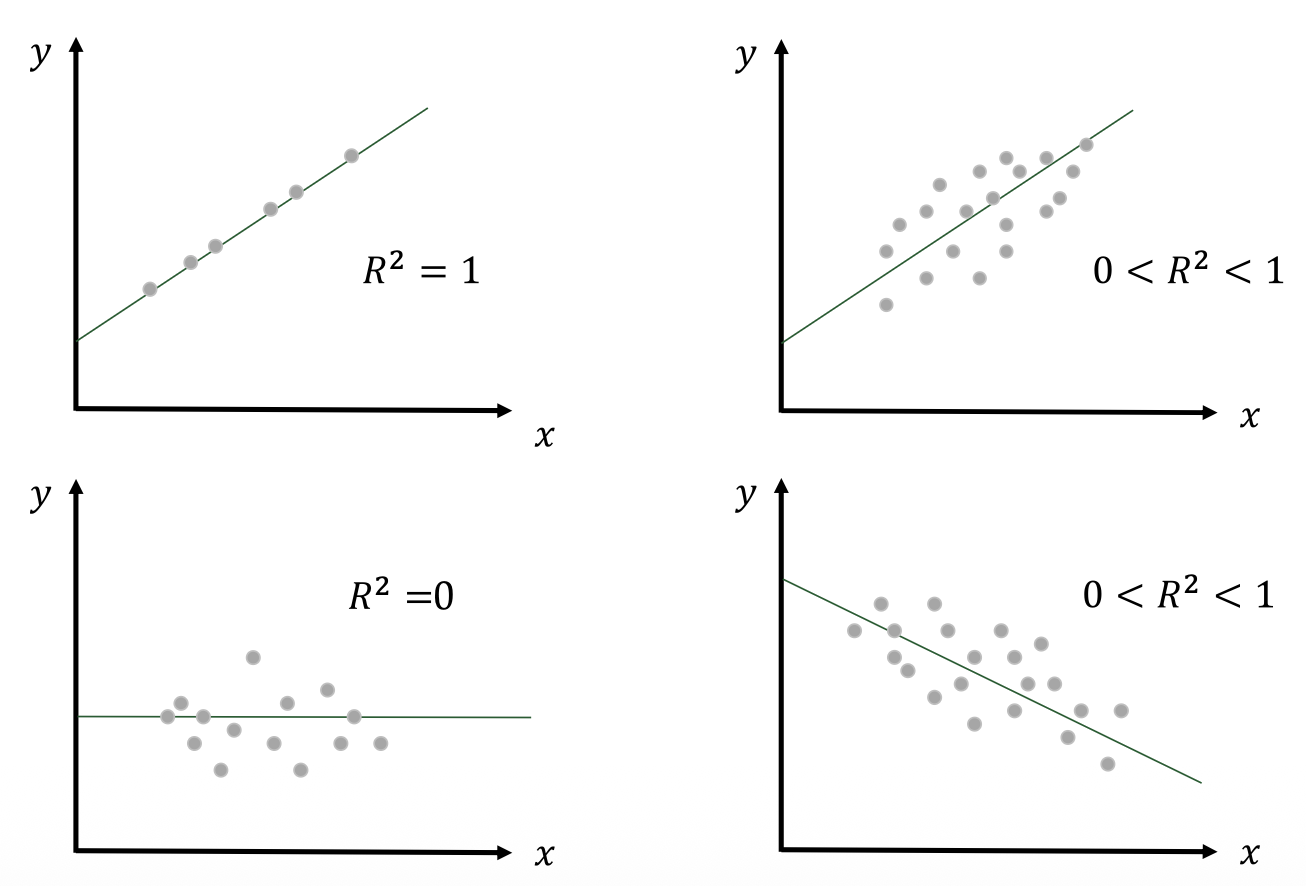
\includegraphics[width=\textwidth]{illustration_verschiedener_bestimmtheitsmasse.png}
		\caption{Illustration verschiedener Bestimmtheitsmasse.}
\end{figure}
\end{definition}

% Zusätzliche Formeln ab S. 22

\section{Multiple Regression}
\subsection{Lernziele}
Nach dieser Vorlesung hat man gelern, wie man die Ergebnisse einer multiplen Regressionsanalyse interpretiert und deren Modellgüte bestimmt wird; man Dummy-Variablen Interaktionseffekte modeliert; potentielle Fehler bei der Regressionsanalyse erkannt und vermieden werden können.

\subsection{Modellannahmen}
Bei der multiplen Regressionsanalyse ergeben sich folgende Notation und Annahmen:

\begin{enumerate}
	\item \text{Annahme:} \(\quad y_{i} = \beta_{1}+\beta_{2} x_{i2} + \beta_{3} x_{i3}+...+\beta_k x_{ik}+e_i \)
	\item \text{Annahme: } \(\quad \mathbb{E}[e_i|x_i]=0 \text{, wobei } x_i=(x_{i2},x_{i3},...,x_{ik})\)
	\item \text{Annahme: } \(\quad \text{Var}(e_i|x_i)=\sigma^2\)
	\item \text{Annahme: } \(\quad \text{Cov}(e_i,e_j|x_i,x_j)=0 \text{ für } i \neq j\)
	\item \text{Annahme: } \(\quad x_i,...,x_n \text{ sind zufällig und nicht kollinear}\)
	\item \text{Annahme: } \(\quad e_i,...,e_n \text{ sind normalverteilt}.\)
\end{enumerate}

\begin{definition}[Adjusted R-Square]
Bei der multiplen Regressionsanalyse funktioniert der \(R^2\) nicht mehr, da er sich bei Hinzunahme zusätzlicher unabhängiger Variablen verbessern kann. Der adjusted R-Square überwindet dies
\[ R^2_{adj}=1-\left[(1-R^2)\frac{n-1}{n-k-1}\right].\]
\end{definition}

Um zu überprüfen, ob das Regressionsmodell insgesamt signifikant ist, bietet sich bei der multiplen Regression der sogenannte F-Test an. Dieser prüft, ob die Vorhersage durch das hinzufügen der unabhängigen Variable verbessert wird. Dem sagt man Test der Steigung. Es geben sich folgende Grössen

\[ \text{Mittlere Quadratische Erklärung.} \qquad MSR=\frac{SSR}{k}  \]
\[\text{Mittlere Quadratische Abweichung:} \qquad MSE=\frac{SSE}{n-k-1}\]
\[ \text{F-Ratio} = \frac{MSR}{MSE}\]

Das F-Ratio wird schliesslich mit dem kritischen Wert \(F_C\) verglichen, welcher einer F-Verteilung mit k und n-k-1 Freiheitsgraden folgt. Wenn das F-Ratio den kritischen Wert übersteigt, ist das Modell signifikant und es können die linearen Zusammenhänge bestätigt werden. Es wird dann also die Nullhypothese \((H_0: \beta_2=\beta_3=\beta_4=...=\beta_k=0)\) widerlegt.

\begin{definition}[Heteroskedastizität]
Bei einer Verletzung von Annahme 3 (\(\text{Var}(e_i|x_i)=\sigma^2\)) liegt Heteroskedastizität vor. Dies ist der Fall, wenn sich die Varianz der Residuen über die abhängige Variable \(x_i\) vergrössert oder verkleinert. Heteroskedastizität ist problematisch, da sie zu einer Fehleinschätzung der Standardfehler der Regressionskoeffizienten führt. Die statistische Signifikanz der Schätzer wird dadurch verzerrt und auch Hypothesentests sowie Konfidenzintervalle werden folglich fehlerhaft.
\end{definition}

\begin{definition}[Autokorrelation]
Im Falle der Autokorrelation ist Annahme 4 (\(\text{Cov}(e_i,e_j|x_i,x_j)=0\)) verletzt. Die Residuen in einer Periode sind dabei mit den Residuen in einer anderen Periode korreliert. Dieses Problem tritt vor allem bei Zeitreihendaten auf. Wie bei der Heteroskedastizität wird dadurch die Signifikanz der OLS Schätzer falsch eingeschätzt.
\end{definition}

\begin{definition}[Multikollinearität]
Bei der Multikollinearität wird Annahme 5 verletzt. Perfekte Multikollinearität liegt dann vor, wenn es eine exakte lineare Beziehung zwischen zwei oder mehreren unabhängigen Variablen gibt. Schwache Multikollinearität entsteht dann, wenn zwei unabhängige Variablen hoch korreliert sind, aber sich nicht gegenseitig bestimmen. Sie stellt kein grosses Problem dar, da die überschüssigen Variablen einfach entfernt werden können. Im Falle der schwachen Multikollinearität erhöhen sich Standardfehler, was durch eine grössere Stichprobe kompensiert werden kann.
\end{definition}

\end{document}